\chapter{绪论}
\label{chap:introduction}

\section{研究背景和意义}
核磁共振成像\cite{mrireview}(magnetic resonance imaging,简称MRI)是医学临床上常用的成像方法,其利用核磁共振现象来实现高对比度成像,可以非侵入式地获取人体内部组织的信息,被广泛地应用于指导病灶检测、诊断与治疗\cite{lustig2006}。MRI在医学临床和研究中有很多不同的分类方式,根据图像是否含有时间维度,可以将MR图像分为静态MR图像和动态MR图像(dynamic MRI,简称dMRI)。常见的动态MRI有心脏电影成像(cardiac cine)、心脏灌注成像(cardiac perfusion)、磁共振动态对比增强(dynamic contrast enhanced MRI,简称DCE-MRI)、功能核磁共振成像(function MRI,简称fMRI)等,如图\ref{fig:dynamic}所示。
\begin{figure}[htbp]
\centering
\subfigure[心脏电影(一帧)]{
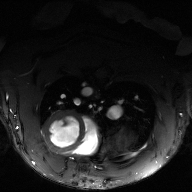
\includegraphics[width=2.11in]{img/intro/cine.png}
}
\subfigure[胸部DCE-MRI(一帧)]{
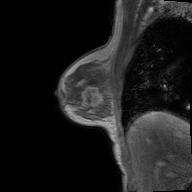
\includegraphics[width=2.11in]{img/intro/breast.png}
}
\subfigure[心脏灌注(一帧)]{
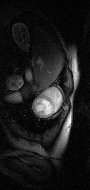
\includegraphics[width=1in]{img/intro/perfusion.png}
}
\centering
\caption{动态MR图像举例。}
\label{fig:dynamic}
\end{figure}

\section{本文的主要研究内容和章节安排}

第二章 ...

第三章 ...

第四章 ...

第五章,我们对本文的工作进行了总结并给出了下一步工作展望。





